\documentclass{ou-report}
\newcommand{\mycomment}[1]{}
\usepackage[acronym, section=sub subsection]{glossaries}
\usepackage{booktabs}
\usepackage{todonotes}
\usepackage{float}
\usepackage{leading}
\usepackage{algorithm}
\usepackage{algpseudocode}
\usepackage{hyperref}

\let\oldFootnote\footnote
\newcommand\nextToken\relax

\renewcommand\footnote[1]{%
    \oldFootnote{#1}\futurelet\nextToken\isFootnote}

\newcommand\isFootnote{%
    \ifx\footnote\nextToken\textsuperscript{,}\fi}
    
\newglossary*{genericmath}{Math symbols}
\newglossary*{2dlaplace}{2D-Laplace symbols}
\makeglossaries
\citestyle{agu}

% Dit template is gemaakt door P.J. Molijn in het kader van zijn afstuderen aan de OU in 2014.
% Waarvoor hartelijk dank.
% Minieme maar belangrijke wijzigingen zijn aangebracht door E.M. van Doorn
% Het template is versimpeld door Sylvia Stuurman, 2019.


%\hypersetup{
%pdfsubject={Master Thesis <Titel>, <author>},
%pdfkeywords={keyword1, keyword2}
%}

\begin{document}
\pagestyle{plain}
\title{Dit is de titel van mijn afstudeerverslag}
\author{Tjibbe van der Ende}
%Title of the thesis
%\title[Subtitle]{Title}
%\author{author}
%\affiliation{
%\begin{tabular}{ll}
%Student: & studentnumber \\
%Date:    & DD/MM/YYY \\
%\end{tabular}
%}
%
%%\coverimage{cover/cover.jpg}
%%            ===============
%\makecover[frontboxwidth=4.6in]
\begin{titlepage}

    \begin{center}

        %% Insert the OU logo at the bottom of the page.
        \begin{tikzpicture}[remember picture,overlay]
            \node at (current page.south)[anchor=south,inner sep=0pt]{
                \includegraphics[scale=0.7]{cover/logo}
            };
        \end{tikzpicture}

        %% Extra whitespace at the top.
        \vspace*{2\bigskipamount}

        %% Print the title in specific color.
        {\makeatletter
            %\titlestyle\color{ou-cyan}\Huge\@title
            \titlestyle\color{red}\Huge\@title
            \makeatother}

        %% Print the optional subtitle in black.
        {\makeatletter
            \ifx\@subtitle\undefined\else
                \bigskip
                \titlefont\titleshape\LARGE\@subtitle
            \fi
            \makeatother}

        \bigskip
        \bigskip

        by
        %door

        \bigskip
        \bigskip

        %% Print the name of the author.
        {\makeatletter
            \titlefont\Large\bfseries\@author
            \makeatother}

        \vfill

        in partial fulfillment of the requirements for the degree of
        %in overeenstemming met de vereisten voor het verkrijgen van de graad van

        \bigskip
        \bigskip

        {\bfseries Master of Science}

        in Software Engineering

        \bigskip
        \bigskip

        at the Open University, faculty of Management, Science and Technology \\
        Master Software Engineering
        %aan de Open Universiteit Nederland,

        to be defended publicly on 12 October, 2023 at 9:30 AM.
        %in het openbaar te verdedigen op dinsdag 9 september om 15:00 uur.

        \vfill

        \begin{tabular}{lll}
            %% Add additional information here, per faculty requirements, e.g
            Student number: & 852372917                                                 \\
            Course code:    & IMA0002                                                   \\
            Thesis committee:
                            & Dr. Ir. Mina Sheikhalishahi (chairman), & Open University \\
                            & Dr. Ir. Clara Maathuis (supervisor),    & Open University
        \end{tabular}

        %% Only include the following lines if confidentiality is applicable.
        \bigskip


        \bigskip

    \end{center}

\end{titlepage}


%% Use Roman numerals for the page numbers of the title pages and table of
%% contents.
\pagenumbering{roman}
%% Include an optional title page.

\frontmatter


\let\cleardoublepage\clearpage

% Optional Dedication, Acknowledgement
%\input{dedication}

%\input{acknowledgement}
\tableofcontents

%Optional: list of figures, list of tables
%\listoffigures

%\listoftables

%% Include an optional summary page.
%\chapter{Summary}
Data has become a crucial part of our daily lives, with personal and sensitive information often sourced from various data sources. As businesses recognize the potential of data, the need for data protection has increased, leading to regulations like the GDPR and the privacy act. Unsupervised machine learning, such as clustering, is used to gain insights into data. However, encryption is unsuitable for data analysis due to its communication overhead and unreadable nature. Anonymization methods have been explored, but they can still reveal personal information. Differential privacy, which adds noise to the original data to hide the actual value, is an effective way to preserve privacy while preserving data patterns. However, this method has limitations, such as leaking distance information and focusing on 2-dimensional synthetic datasets. The research aims to develop a privacy framework that enables secure training of various clustering algorithms on distributed n-dimensional data, addressing the shortcomings of previous studies and real-world dataset challenges. \newline

This thesis aims to develop a new privacy framework for training clustering algorithms on distributed n-dimensional data. It aims to extend the use of \gls{gi} to optimize specifically the clustering of data. The proposed method relies on distance-based considerations, ensuring the shape and structure of the data are preserved during the clustering process. The thesis includes a research question titled "How can the nD-Laplace mechanism be applied in training privacy-preserving clustering algorithms on distributed n-dimensional data?" and a series of experiments using real-world datasets and synthetic datasets. The research uses both external and internal validation methods to assess the utility and privacy of the privacy mechanism. The qualitative data from these experiments is analyzed to compare various privacy mechanisms and their performance concerning clustering tasks.
%\input{Summary/samenvatting}

\newglossaryentry{ari}{type=\acronymtype, name={ARI}, description={Adjusted Rank Index}, first={Adjusted Rank Index (ARI)\glsadd{arig}}, see=[Glossary:]{arig}}
\newglossaryentry{ami}{type=\acronymtype, name={AMI}, description={Adjusted Mutual Information}, first={Adjusted Mutual Information (AMI)\glsadd{amig}}, see=[Glossary:]{amig}}
\newglossaryentry{ldp}{type=\acronymtype, name={LDP}, description={Local Differential Privacy}, first={Local Differential Privacy (LDP)}}
\newglossaryentry{dp}{type=\acronymtype, name={DP}, description={Differential Privacy}, first={Differential Privacy (DP)}}
\newglossaryentry{bv}{type=\acronymtype, name={BV}, description={Bit Vector}, first={Bit Vector (BV)}}
\newglossaryentry{nmi}{type=\acronymtype, name={NMI}, description={Normalized Mutual Information}, first={Normalized Mutual Information (NMI)\glsadd{nmig}}, see=[Glossary:]{nmig}}
\newglossaryentry{dbscan}{type=\acronymtype, name={DBSCAN}, description={Density-based spatial clustering of applications with noise}, first={Density-based spatial clustering of applications with noise (DBSCAN)}}
\newglossaryentry{aee}{type=\acronymtype, name={AEE}, description={Average Estimated Error}, first={Average Estimated Error (AEE)\glsadd{aeeg}}, see=[Glossary:]{aeeg}}
\newglossaryentry{mi}{type=\acronymtype, name={MI}, description={Mutual Information}, first={Mutual Information (MI)\glsadd{mig}}, see=[Glossary:]{mig}}
\newglossaryentry{chi}{type=\acronymtype, name={CHI}, description={Calinski-Harabasz Index}, first={Calinski-Harabasz Index (CHI)\glsadd{chig}}, see=[Glossary:]{chig}}
\newglossaryentry{gi}{type=\acronymtype, name={GI}, description={Geo-indistinguishability}, first={Geo-indistinguishability (GI)}}
\newglossaryentry{ap}{type=\acronymtype, name={AP}, description={Affinity Propogation}, first={Affinity Propogation (AP)}}
\newglossaryentry{dpc}{type=\acronymtype, name={DPC}, description={Density Peaks Clustering}, first={Density Peaks Clustering (DPC)}}
\newglossaryentry{birch}{type=\acronymtype, name={BIRCH}, description={Balanced Iterative Reducing and Clustering using Hierarchies}, first={Balanced Iterative Reducing and Clustering using Hierarchies (BIRCH)}}
\newglossaryentry{optics}{type=\acronymtype, name={OPTICS}, description={TODO}}
\newglossaryentry{pdf}{type=\acronymtype, name={PDF}, description={Probability Density Function}, first={Probability Density Function (PDF)}}
\newglossaryentry{pm}{type=\acronymtype, name={PM}, description={Piecewise Mechanism}, first={Piecewise Mechanism (PM)}}
\newglossaryentry{svm}{type=\acronymtype, name={SVM}, description={Support Vector Machine}, first={Support Vector Machine (SVM)}}
\newglossaryentry{cdf}{type=\acronymtype, name={CDF}, description={Cumulative Distribution Function}, first={Cumulative Distribution Function (CDF)}}
\newglossaryentry{mia}{type=\acronymtype, name={MIA}, description={Membership Inference Attack}, first={Membership Inference Attack (MIA)}}
\newglossaryentry{tpr}{type=\acronymtype, name={TPR}, description={True Positive Rate}, first={True Positive Rate (TPR)}}
\newglossaryentry{fpr}{type=\acronymtype, name={FPR}, description={False Positive Rate}, first={False Positive Rate (FPR)}}
\newglossaryentry{rig}
{
	name=Rand Index,
	description={
			Compares the similarity between two clusters by comparing all pairs.
			It can therefore be used to measure the performance between two clustering algorithms \citep{hubert_comparing_1985}. }
}
\newglossaryentry{arig}
{
	name=Adjusted Rand Index,
	description={
			The Rand Index is improved and adjusted for chance \citep{hubert_comparing_1985}.
			This algorithm takes also into consideration the number of clusters and can be used to also compare different cluster algorithms \citep{gates_impact_2017}.}
}
\newglossaryentry{mig}{
	name=Mutual Information,
	description={This metric can be used to explain the amount of information about a random variable if compared to another random variable.
			Therefore, it can also be used to compare two cluster similarities.}
}
\newglossaryentry{amig}{
	name=Adjusted Mutual Information,
	description={Comparable with \gls{arig} this algorithm is modified to account to chance.
			This means it accounts for a higher MI for a higher amount of clusters between two cluster algorithms. Therefore, the calculations are strongly influenced by that of \gls{arig} \citep{vinh_information_2009}. }
}


\newglossaryentry{nmig}{
	name=Normalized Mutual Information,
	description={The normalized version is a scaled version of \gls{mig} to always be a value between 0 (no correlation) and 1 (perfect correlation).
			This version of \gls{mig} is not adjusted and therefore highly influenced by cluster amount \citep{vinh_information_2009}. So it suffers the same issue as with \gls{mig}.}
}

\newglossaryentry{bvg}{
	name=Bit Vector,
	description={List or array to store several bits.}
}

\newglossaryentry{aeeg}{
	name=Average Estimation Error,
	description={This is the difference between an estimated value and the real value.}
}

\newglossaryentry{chig}{
	name=Calinski-Harabasz Index,
	description={This is a way to measure the similarity of clusters \citep{calinski_dendrite_1974}.
			It tells how well the clusters are separated from each other and how well the points are grouped.}
}

\mainmatter
\pagenumbering{arabic}

\chapter{Title of the chapter}
This is just to show how to include a test file for a chapter, a reference \cite{ledesma_scree_2015}

\chapter{Literature review}
The current chapter explains the theoretical aspects of the research and evaluates similar and previous studies.
First, the concept of Differential Privacy and its various types is explained.
Next, we examine cluster algorithms and the methods for evaluating their performance.
Regarding the related literature, we first look at studies that have used differential privacy and then the studies that have combined it with cluster methods.

\section{Differential privacy}
\subsection{Laplace algorithm}
\subsection{Local differential privacy}
\subsection{Evaluation methods}
Is also possible to evaluate and measure the impact of the noise between two distributions.

\todo[inline]{RE versus other methods}

\section{Clustering}

\subsection{Methods}
\todo[inline]{Describe each clustering method with important parameters that could influence the outcome}
\subsubsection{K-Means} \label{theory:kmeans}
\todo[inline]{Explain the working of the algorithm}.
The most important parameter of the K-Means algorithm is the value of $k$.
This value determines the number of clusters to consider and has a big influence on the results \cite{ahmed_k-means_2020}.
One of the oldest methods to do this is to use an "elbow" plot \cite{kodinariya_review_2013}.
This method can be used to determine the best $k$ by applying the algorithm multiple times and estimateing the best $k$.
\begin{figure}[H]
  \includegraphics{TheorethicalFramework/dentification-of-Elbow-point.png}
  \caption{Illustration of determining $k$ using the "elbow" method \cite{kodinariya_review_2013}}
\end{figure}
However, sometimes the "elbow" is hard to find

\subsubsection{Affinity Propagation}:
\todo[inline]{Explain the working of the algorithm}.
\todo[inline]{Explain most important parameters}
\subsubsection{DBSCAN}:
\citep{bozdemir_privacy-preserving_nodate}
\todo[inline]{Explain the working of the algorithm}.
\todo[inline]{Explain most important parameters}

\subsection{Evaluation methods} \label{theory:evaluate}
Clustering comparison measures are important in cluster analysis for external validation by comparing clustering solutions to a "ground truth" clustering \citep{vinh_information_nodate-2}.
These external validity indices are a common way to assess the quality of unsupervised machine learning methods like clustering \citep{warrens_understanding_2022}.
A method that could be used for this is the Rand Index \citep{rand_objective_1971}.
It is a commonly applied method for comparing two different cluster algorithms \citep{wagner_comparing_nodate}.
An improvement of this method is adjusted for chance by considering the similarity of pairwise cluster comparisons \citep{vinh_information_nodate-2}.
Both the Rand Index (RI) and Adjusted Rand Index (ARI) \citep{hubert_comparing_1985-1} report a value between 0 and 1.
Where 0 is for no-similarity and 1 for identical clusters.
Alternatives for RI are the Fowles-Mallows Index and Mirkin Metric.
However, these two methods have their disadvantages. Respectively, being sensitive to a few clusters and cluster sizes \citep{wagner_comparing_nodate}.
The ARI metric suffers from cluster size imbalance as well, so it only provides not a lot of information on smaller clusters \citep{warrens_understanding_2022}.
Instead, they recommend using the cluster index metric that was proposed by Fränti et al. \citep{franti_centroid_2014}.

Another popular group of methods is the information theoric-based measures \citep{vinh_information_nodate-2}.
This metric measures the information between centroids; the higher the value, the better \citep{vinh_information_nodate-2}.
\gls{mi} is such metric, which calculates the probability of an element belonging to cluster $C$ or $C`$.
But, is not easy to interpret as it does not have a maximum value \citep{wagner_comparing_nodate}.
To this end, \gls{nmi} can be used to report a value between 0 and 1 using the geometric mean \citep{strehl_cluster_2002}.
The metric exists also in an adjusted version as \gls{ami}.
This works in the same way as for the \gls{ari} and is mostly needed if the number of data items is small in comparison to the number of clusters \citep{vinh_information_nodate-2}. \newline

Besides the external validity measurements for clustering, it is also possible to use internal validation methods.
These metrics focus entirely on the intrinsic dataset properties, instead of relying on an external baseline cluster algorithm \cite{craenendonck_using_nodate}.
Assessing two important concepts of clustering: compactness and separation \cite{hassani_using_2017}.
Both studies, consider three different metrics and measure both concepts at the same time \cite{hassani_using_2017}:
\begin{enumerate}
  \item \gls{chi} \citep{calinski_dendrite_1974-1} is used to measure the cluster variance (well-separated clusters) and low variance within the clusters (tightly coupled data). A high score indicates better clustering.
  \item Silhouette Index \citep{rousseeuw_silhouettes_1987} this metric is similar, by also measuring cohesion within clusters and separation of clusters. However, this metric uses the pairwise distance \cite{hassani_using_2017}. A score of -1 indicates incorrect clustering and +1 for dense clusters \cite{rousseeuw_silhouettes_1987}.
  \item Davies-Bouldin \citep{davies_cluster_1979} uses the average distance between centroids. A lower score indicates good clustering.
\end{enumerate}

K-Means scores relatively high for \gls{chi} \citep{craenendonck_using_nodate,hassani_using_2017} and SI \citep{craenendonck_using_nodate}.
The same applies to DBSCAN, which scores relatively high on SI and DB due to the sensitivity of noise \cite{craenendonck_using_nodate}.
% Thus, these metrics are difficult to use for very different cluster algorithms \cite{craenendonck_using_nodate}.
\subsubsection{Existing literature}
%A recent and much-cited study uses \gls{ari} and accuracy as metrics for evaluating K-Means \cite{ahmed_k-means_2020}.
%The accuracy is measured by calculating the percentage of the correct predicted labels and their truth labels.
Comparable studies with differential privacy use external validation \citep{xia_distributed_2020-1, sun_privbv_2022}.
Their experiment setup uses a so-called non-private cluster algorithm as external validation.
This cluster algorithm is trained without the perturbed data and compared with the same clustering algorithm that is trained with perturbed data.
Thus, the non-private variant functions as an external validation by providing the ground truth.

They compare the mutual information between a baseline cluster algorithm using \gls{ami} \citep{9679364} or \gls{nmi} \citep{xia_distributed_2020-1,sun_privbv_2022}.
Another study for evaluating \gls{dp} with \gls{ap} uses both \gls{ari} and \gls{ami}.
In addition to mutual information and rand index scores, it is also not uncommon to calculate the error between the two cluster algorithm's centroids \citep{xia_distributed_2020-1, 9679364}.
These two studies used Relative Error (RE) for this.
\section{Literature review} \label{theory:literature-review}
The related literature is divided into three parts:
\begin{enumerate}
  \item Differential privacy methods
  \item Cluster methods with (L)DP
\end{enumerate}
Afterward, we provide a summary for both in the form of a table.
This table includes components such as the type (LDP or DP) and whether there is a public code available.

\subsection{Differential privacy methods}
As was discussed in earlier sections, the Laplace method was the first one to establish \gls{dp} \citep{dwork_differential_2006}.
In the search for related literature, research has mainly focused on algorithms that can be used for general applications.
This includes investigating whether the mechanisms can also be applied to n-dimensional data, as is the case with our mechanism.

The first paper is provided by Soria-Comas et al. and considers the distribution of the dataset for the provided noise \citep{soria-comas_optimal_2013}.
It does however not depend on the data and does not calibrate sensitivity.
Their work claims the Laplace mechanism is not optimal for a univariate function and aims at improving it by introducing their Laplace-based mechanism.
The method that is proposed performs slightly better than Laplace.
For multivariate/multiple queries the Laplace distribution underperforms.

Quan et al. also proposed a new method as an extension of Dwork et al.'s Laplace algorithm \citep{geng_staircase_2013}.
They introduced the staircase mechanism for 1-dimensional noise, which was later extended to support multidimensional data \citep{geng_staircase_2015}.

The mechanism aims to improve optimally by adding the same level of privacy while adding less noise.
It is represented as a staircase-shaped probability density function, hence the name Staircase Mechanism (SM).
This mechanism accepts three configurable parameters, which are comparable to those of the Laplace mechanism.
The authors' work can handle multidimensional numerical data and preserve the pure version of differential privacy.
%One disadvantage of the staircase mechanism is that it can produce an unbounded output, as noted by Wang et al. 
%This means that the perturbed data can exceed the original bounds of the data. 
%Additionally, the authors do not compare their results to comparable work in an experimental setting.

Another paper introduces a new local differential privacy (LDP) mechanism for working with numerical data \citep{nguyen_collecting_2016}
Their primary focus is on estimating means and frequencies, with a particular emphasis on machine learning techniques such as Support Vector Machines (SVM) and linear regression using Empirical Risk Minimization.
Initially, the authors analyze Duchi et al.'s method \citep{duchi_privacy_2013} and highlight several shortcomings.
To address these issues, they introduce Harmony as a mechanism for LDP perturbation. Additionally, they extend other work (Bassily and Smith's method) to introduce a method for perturbing multi-dimensional categorical attributes.
The authors then create a hybrid model by combining Duchi et al.'s method and Bassily and Smith's method to handle respectively numeric and categorical data. This allows them to compare their method Harmony to the hybrid mechanism and measure the utility/accuracy differences.

Duchi et al. improved their method by proposing a formalization of the trade-off between statistical utility and (local) privacy, analyzing multiple types of estimation problems \citep{duchi_minimax_2017}.
Examples include mean, median, and density estimation.
To achieve this, they use minimax, a technique for finding the worst-case probability distribution [Minimax].
Additionally, they focus on existing work and propose several optimization strategies for it.

This work extends the method proposed in the previous paragraph by Duchi et al. by adding support for bounded and multidimensional data \citep{wang_collecting_2019}.
The authors introduce the Piecewise Mechanism (PM) to handle both numeric and categorical data and the Hybrid Mechanism (HM) which combines PM and Duchi et al.'s method for 1-dimensional data.
The effectiveness of their method is demonstrated using Support Vector Machines (SVM), linear regression, and mean estimation.
PM and HM are compared to Laplace, SCDF \todo{bron}, and Duchi et al.'s solutions.
OUE \todo{bron} is also used for comparison, but for categorical data only, as this is not supported by the other methods.
% Instead of using the aforementioned techniques, categorical data is compared using frequency counting.


%\subsection{Geo-indistinguishability methods}
%\todo[inline]{Currently still work in progress}
\subsection{Cluster methods with (L)DP}
This chapter examines the various studies that have been conducted on clustering in combination with differential privacy.
Initially, we looked at the most fundamental papers in this field. Subsequently, the focus shifted toward researching well-known papers that have been published since 2020.

The work that was proposed by Nissim et al. aims to improve differential privacy methods, such as Laplace, which use sensitivity to compensate the noise for a function.
In addition to compensating the function, they also consider the dataset itself.
The algorithm for this is called "smooth sensitivity" and is used for instance-specific noise.
To apply it, the authors introduce a method/framework to effectively calculate it.
To demonstrate the effectiveness of the method, they use K-means, among other cluster algorithms.
Their method requires the calculation of cluster distances, using Wasserstein distance instead of Euclidean distance.
%Although, it preserves $(\epsilon, \delta)$-LDP it does not provide any experiments with real world datasets.

Another study focuses on both interactive and non-interactive approaches for differential privacy in K-Means \citep{su_differentially_2015-1}.
The study builds upon the work done for DPLloyd, an interactive privacy extension of K-Means described by Blum et al. \citep{blum_practical_2005}.
The DPLLoyd mechanism partitions an n-dimensional dataset into a grid and releases the count for each grid by adding Laplacian noise to each count.
Another part of their research focuses on determining the width of the data cells.
The grid estimation method used in their research is called the extended uniform grid approach (EUG), and the complete K-Means method is called EUGkM.
The experiment consists of comparing against the DPLloyd mechanism, which performs better for an interactive setting.
Therefore, they combine their algorithm for combining both aspects into a hybrid approach (EUGkM + DPLloyd approach) and show a better final performance.

The study of Nissim et al. researches the idea of finding the smallest possible radius in the Euclidean space  $R^d$ for a set of $n$ points \citep{nissim_clustering_2018}.
They propose a new solution that uses locality-sensitive hashing (LSH) for differential privacy, which they use to find 1-cluster in the $d$-dimensional Euclidean space.
This method works for differential privacy (LSH-GoodCenter), but they also extend this to the local model (LDP-GoodCenter).
The algorithm to find this radius is used to count the points enclosed by the radius and Laplace noise is added to the count to preserve differential privacy.
This mechanism is combined and applied to work with the K-Means algorithm (LDP-K-Mean).
This method was later extended in a paper proposed by Kaplan et al. and introduces a similar LDP method \citep{kaplan_differentially_2018}.
They aim to reduce the number of interactions needed between the server and users to one, instead of the $O(k\log n)$ required for Nissam et al.’s solution \citep{nissim_clustering_2018}.
To increase the success probability, they use the same idea but extend it to have multiple centers instead of one large one.
They call it the LSH-Procedure and the algorithm Private-Centers is applied to generate centers to use with K-Means.
Then, they apply the same method to the LDP method that was also originally proposed by Nissam et al. (LDP-GoodCenter).
The most recent work by Stemmer et al. focuses on improving the work that was done by Kaplan et al. \citep{kaplan_differentially_2018,stemmer_locally_2021}.
Because this work has a higher additive error, which means the noise that is added introduces a lot of error.
To solve this, the authors aim at reducing this error by improving the original GoodCenter algorithm \citep{nissim_clustering_2018}.
Their extended method is called WeightedCenters and adds weights to candidate centers.
So, in addition to calculating the centroids for each iteration, it also calculates the weights for each.
In the final iteration, the weights are used to create the K-Means or K-Median clusters.

Sun et al. proposed a method for distributed clustering using local differential privacy (LDP) to preserve distance-based information.
They claim to have the first non-interactive LDP algorithm for clustering \citep{sun_differentially_2019}.
This means, they are being able to perturb the data locally at once and sent it to the server to cluster with both K-Means and DBSCAN.
They encode the client-side data into an anonymous hamming space using Bit Vector (BV) and modify the encoding to preserve Euclidean distance.
As their method only is be-able to share distance information they were not able to use K-Means directly. To overcome this, they modified the algorithm and called it K-Cluster.
Finally, the method is evaluated using Normalized Mutual Information (NMI) and Average Estimated Error (AEE).
\todo[inline]{PrivBV}

Xia et al. noticed the shortcoming of Sun et al.'s work which is the need to share privacy-sensitive distance information \citep{xia_distributed_2020-1}.
Therefore, they propose a new interactive method for distributed K-means clustering using LDP.
The method converts features to binary strings and uses a Random Response mechanism (RR) to perturb each feature into a feature vector.
The privacy cost depends on the length of the bits of each feature transformation, meaning that a longer length yields more information at the cost of the privacy budget.
In each iteration, the server-side calculates and sends K-means centroids to each user, who recalculates distances until the centroids become stable.
The approach has the disadvantage of a high correlation between user data and the clusters.
To solve this problem, the algorithm is improved by having the client-side send not only the user data but also a set of random zero strings.
The server side then performs similar calculations to determine the true cluster.
Huang et al. propose a private distributed K-means clustering algorithm for interval data that addresses a shortcoming in Xia et al.'s work by using Condensed Local Differential Privacy (CLDP) for small-scale values and LDP for large-scale values \citep{9679364}.
They preserve distance using a Square Wave (SW) mechanism and apply a classical K-Means algorithm on the server side to the perturbed data.

Another more recent mechanism that also builds around K-Means to preserve LDP, is called the LDPK mechanism \citep{yuan_privacypreserving_2021}.
As K-Means works only with numerical data, they use K-prototypes for supporting mixed data types.
The LDPK mechanism perturbs the user data first locally and interactively exchanges information with the server to complete the clustering process.
The mechanism they use for perturbation is the Harmony algorithm, which was proposed earlier by \citep{nguyen_collecting_2016}.
To also support categorical data the S-Hist method is used, which was also introduced by Nguyen et al.
But the author replaces this algorithm with OUE \cite{wang_locally_nodate} to improve accuracy.
Due to the correlation between the cluster centroids and the real data, the server could still infer the correct information.
Therefore, the authors also disturb the user’s cluster information with an extra extension to the LDPK method, called ELDPK.
To this end, they perturb the clusters with the GRR (Generalized Random Response) algorithm.
Their evaluation focuses on the privacy budget and the amount of data points.
They show that if the amount of data points increases the clustering quality does as well. \newline

The conclusion from the previous paragraphs is that most of the related work focuses on variants of the K-Means algorithm.
Finally, two interesting studies focus on differential privacy and \gls{ap} or \gls{dbscan}.
A study conducted by Cai et al. focuses on \gls{ap} \citep{cai_dp-ap_2020}.
Their method involves adding Laplace noise to the responsibility matrix.
For each sample data, a neighborhood is specified using a radius around the data point.
This area is called the neighborhood density, and each sample point’s preference value is adjusted according to its density value.
Higher density yields a higher chance of belonging to a cluster center and then being ranked based on size.
The perturbed responsibility matrix and densities are combined and used to run AP.
Finally, they evaluated their method using the  \gls{ari}, Fowlkes-Mallows Index (FMI), and \gls{ami}.

Another recent study focuses on differential privacy for \gls{dbscan} \citep{bozdemir_privacy-preserving_nodate}.
The proposed solution involves clustering data between two or more parties using two servers.
Secure two-party computation (S2PC) is used to achieve this.
Using S2PC, both servers receive a random-looking secret share.
To recover the original data, both servers would need to combine their shares using S2PC, which combines the data without the servers having access to the full value.
The proposed protocol is named privacy-preserving \gls{dbscan} (ppDBSCAN).
The calculations in this study are based on squared Euclidean distance (SED) and are evaluated using different methods.
To evaluate the performance of ppDBSCAN, the study compares its Adjusted Rand Index (ARI) to that of K-means.

\subsection{Summary}
\todo[inline]{Short summary}
\begin{landscape}
  \begin{table}[ht]
    \centering
    \begin{adjustbox}{width=1.8\textwidth}
      \begin{tabular}{rlllllllll}
        \toprule
        year              & Name                                                                                                          & Data type                            & Dataset                                            & Code implementations                    & preserving                 & Type                & Interactive     & Methods                                   & Privacy                                                                                                       \\
        \midrule
        2022              & PrivBV: Distance-aware encoding for distributed...                                                            & -                                    & Synthetic dataset                                  & -                                       & Local differential privacy & K-Means             & Non interactive & -                                         & \$(\textbackslash epsilon, \textbackslash delta)\$-LDP                                                        \\
        2021              & Private distributed K-means clustering on inter...                                                            & -                                    & ??                                                 & -                                       & Local differential privacy & K-Means             & Interactive     & -                                         & -                                                                                                             \\
        2021              & Locally Private k-Means Clustering                                                                            & numerical                            & -                                                  & -                                       & Local differential privacy & K-Means             & Interactive     & -                                         & -                                                                                                             \\
        2021              & Privacy‐preserving mechanism for mixed data clu...                                                            & n-dimensional numeric \& categorical & Adult dataset, US Census dataset                   & -                                       & Local differential privacy & K-Prototypes        & Interactive     & LDPK and ELDPK                            & LDP                                                                                                           \\
        2021              & Privacy-preserving Density-based Clustering                                                                   & -                                    & Deer dataset, Lsun dataset, S1                     & -                                       & Differential privacy       & DBSCAN              & -               & ppDBSCAN                                  & -                                                                                                             \\
        2020              & DP-AP: Differential Privacy-Preserving Affinity...                                                            & -                                    & Iris dataset, Seeds dataset                        & -                                       & Differential privacy       & AffinityPropagation & -               & DP-AP                                     & -                                                                                                             \\
        2020              & Distributed K-Means clustering guaranteeing loc...                                                            & n-dimensional numerical data         & 3D Road Network, CarGPS                            & -                                       & Local differential privacy & K-Means             & Interactive     & LDPKmeans                                 & -                                                                                                             \\
        2019              & Distributed Clustering in the Anonymized Space...                                                             & n-dimensional numerical data         & Aggregation dataset, Digit dataset, Pathbased d... & -                                       & Local differential privacy & DBSCAN, K-Means     & Non interactive & Distance Aware Bit Vector (DPBV)          & -                                                                                                             \\
        2018              & Clustering algorithms for the centralized and l...                                                            & n-dimensional numerical data         & -                                                  & -                                       & Local differential privacy & K-Means             & Interactive     & LDP-GOODCenter                            & \$(\textbackslash epsilon, \textbackslash delta)\$-LDP and \$(\textbackslash epsilon, \textbackslash delta... \\
        2018              & Differentially private K-means with constant mu...                                                            & -                                    & -                                                  & -                                       & -                          & K-Means             & Interactive     & - LSH-Procedure
        - Private-Centers & \$(\textbackslash epsilon, \textbackslash delta)\$-DP, \$(\textbackslash epsilon, \textbackslash delta)\$-LDP                                                                                                                                                                                                                                                                                                                                                                        \\
        2015              & Differentially Private k-Means Clustering                                                                     & 2 - 10-dimensional numerical data    & Adult dataset, Gowalla dataset, Image dataset, ... & https://github.com/DongSuIBM/PrivKmeans & Differential privacy       & K-Means             & Both            & EUGkM and hybrid EUGkM + DPLloyd          & -                                                                                                             \\
        %2011              & Differential privacy for location pattern mining                                                              & 2-dimensional geographical data      & Synthetic dataset with GPS trajectories            & -                                       & Differential privacy       & DBSCAN              & -               & DPQuadTree                                & -                                                                                                             \\
        2011              & Smooth sensitivity and sampling in private data...                                                            & n-dimensional numeric                & -                                                  & -                                       & Local differential privacy & K-Means             & Non interactive & Smooth sensitivity for K-Means clustering & \$(\textbackslash epsilon, \textbackslash delta)\$-LDP                                                        \\
        \bottomrule
      \end{tabular}
    \end{adjustbox}
    \caption{Summary table of the literature review for (L)DP clustering algorithms.}
  \end{table}


  \begin{table}[ht]
    \centering
    \begin{adjustbox}{width=1.8\textwidth}

      \begin{tabular}{rlllllllll}
        \toprule
        year                   & Name                                               & Data type                                          & Dataset                                            & Code implementations                               & preserving                 & Type                        & Interactive     & Methods                    & Privacy                         \\
        \midrule
        %2022                    & 3D Geo-Indistinguishability for Indoor Location... & 3-dimensional geographical data                    & -                                                  & -                                                  & Geo-indistinguishability   & Differential privacy method & -               & 3-dimensional Laplace mechanism & -                               \\
        %2019                    & Generalised Differential Privacy for Text Docum... & n-dimensional (?? data)                            & -                                                  & -                                                  & Differential privacy       & Differential privacy method & -               & n-dimensional Laplace mechanism & -                               \\
        2019                   & Collecting and Analyzing Multidimensional Data ... & n-dimensional (PM), but HM is 1-dimensional and... & BR, MR                                             & -https://github.com/forestneo/sunPytools/blob/m... & Local differential privacy & Differential privacy method & -               & - Piecewise Mechanism (PM)
        - Hybrid Mechanism ... & -                                                                                                                                                                                                                                                                                                                                                             \\
        2017                   & Minimax optimal procedures for locally private ... & 1-dimensional numerical data                       & -                                                  & https://github.com/forestneo/sunPytools/blob/ma... & Local differential privacy & Differential privacy method & -               & -                          & -                               \\
        2016                   & Collecting and analyzing data from smart device... & numerical, binary and categorical data. Domain ... & BR (4M records 12 categorical and 6 numeric), U... & -                                                  & Local differential privacy & Differential privacy method & -               & Harmony                    & \$\textbackslash epsilon\$-LDP  \\
        2015                   & The staircase mechanism in differential privacy    & n-dimensional numerical data                       & -                                                  & https://github.com/IBM/differential-privacy-lib... & Differential privacy       & Differential privacy method & -               & Staircase mechanism (SM)   & -                               \\
        2013                   & Optimal data-independent noise for differential... & n-dimensional                                      & -                                                  & -                                                  & Differential privacy       & Differential privacy method & Non interactive & -                          & \$(\textbackslash epsilon)\$-DP \\
        %2012                    & Geo-indistinguishability: Differential privacy ... & 2-dimensional geographical data                    & -                                                  & -                                                  & Geo-indistinguishability   & Differential privacy method & -               & 2-dimensional Laplace mechanism & -                               \\
        \bottomrule
      \end{tabular}
    \end{adjustbox}
    \caption{Summary table of the literature review for (L)DP algorithms.}
  \end{table}
\end{landscape}

\subsection{Evaluation}
It is important to compare our nD-Laplace method with other studies for this research.
Studies that are similar to ours utilize \gls{ldp} for clustering and add noise to cluster centroids \citep{xia_distributed_2020, yuan_privacypreserving_2021, 9679364} or require modifications of the K-Means algorithm \citep{sun_distributed_2019}.

As explained in Section \ref{theory:literature-review:dp-clustering}, we will use input-perturbation.
So, our methodology remains independent of the specific clustering algorithm chosen.
Based on the literature study, two privacy mechanisms are comparable for this approach: Harmony \citep{nguyen_collecting_2016} and Piecewise \citep{wang_collecting_2019}.

Both mechanisms focus on solving the problem in Duchi et al.'s paper.
However, the Harmony mechanism focuses on solving a paper from 2013 \citep{duchi_privacy_2013} and the Piecewise mechanism on Duchi et al.'s paper from 2017 \citep{duchi_minimax_2017}.
The Piecewise mechanism is newer, and given the similarities, Wang et al.'s paper appears much like a more recent version of Nguyen et al.'s paper.
Therefore, we only selected Piecewise to compare with our mechanism.

\subsubsection{Duchi et al.'s mechanism}
The Piecewise mechanism is based on Duchi et al.'s mechanism for one-dimensional data.
Therefore, we start by explaining this mechanism first.
Duchi et al.'s mechanism is a relatively simple method based on the Bernoulli distribution \citep{duchi_minimax_2017}.
This distribution yields either a 0 (negative) or a 1 (false) based on specified probabilities \footnote{https://mathworld.wolfram.com/BernoulliDistribution.html}.
The mechanism works on a domain tuple [-1, 1] and returns -1 or 1.
So, the \gls{pdf} of this function is as follows \footnote{https://mathworld.wolfram.com/BernoulliDistribution.html}:
\begin{equation}[H]
  P(n) =
  \begin{cases}
    1 - p & \text{if } n = 0 \\
    p     & \text{if } n = 1
  \end{cases}
\end{equation}
The probabilities are calculated based on the input value and can then be used to estimate a mean value.
Compared to Laplace, Duchi et al. solution performs better in variance for epsilons smaller than 2 \citep{wang_collecting_2019}.
However, it performs worse when the epsilon value is higher because the algorithm does not consider the privacy budget for values that are 0.
The multidimensional variant looks like the one-dimensional version but samples each data point's noise independently.

\subsubsection*{Piecewise mechanism} \label{theory:piecewise}
The authors aim to create a method that combines the advantages of the Laplace mechanism and Duchi et al.'s methods \citep{wang_collecting_2019}.
The goal is to reduce the variance for a broader range of privacy budgets.
Like the mechanism above, the Piecewise mechanism only accepts data from -1 to 1.
We first explain the one-dimensional variant and then the multidimensional variant. \newpage

The mechanism takes an input of the range $[-1, 1]$ and returns a perturbed value in the same range.
It uses a piecewise function (hence the name), which is a function that is defined by multiple sub-functions.
The Piecewise mechanism starts with randomly selecting a value $x$ between 0 and 1 and a value $t \in R^1$.
Then, based on this value the mechanism re-assigns a random value to $x$, but with a modified domain (based on the initial value of $x$) \citep{wang_collecting_2019}:
\begin{equation} \label{eq:piecewise-domain}
  t = \begin{cases}
    [l(t), r(t)] & \text{if } x < \frac{e^{\epsilon/2}}{e^{\epsilon/2}+1} \\
    [-C, l(t) \cup r(t), C]
  \end{cases}
\end{equation}
%According to this formula, the outcome domain shifts depending on the value of $t$.
\begin{enumerate}
  \item Calculated using the privacy budget $\epsilon$, the $C$ determines the amount of noise by bounding the lower/ upper limit of the domain.
  \item $l(t)$ and $r(t)$ are the left and right boundaries of the domain. These are calculated based on the value of $t$ and the privacy budget.
\end{enumerate}
Depending on the value of $t$, the domain is shifted to the left or right on a domain of three "pieces": $[-1, 0, 1]$ \citep{wang_collecting_2019}.
According to Wang et al., when $t = 0$, the probability of $t \in [l(t), r(t)]$ is higher.
In this case, the mechanism generates a perturbed value close to $0$ (depending on the privacy budget).
This phenomenon is the same for $t = 1$ and $t = -1$. \newline
%Where $C$ is defined according to the following mathematical formula:
%\begin{equation}
%  C = \frac{exp(\epsilon/2)+1}{exp(\epsilon/2) - 1} \\
%  \label{fig:piecewise-C}
%\end{equation}
%The noise is sampled from this distribution by conditionally executing one of two algorithms (see for reference Wang et al.'s paper) \citep{wang_collecting_2019}.

%Due to the symmetric nature of their mechanism's \gls{pdf}, the authors can handle the value of 0.
%Imagine it as a histogram with the distribution centered around 0. \todo[inline]{mathematical formula?}
%The histogram consists of three "parts" on the left, right, and center (0).
%This approach allows for determining the probability of 0 based on a certain likelihood, unlike Duchi et al.'s solution.

For multidimensional data, the authors use the one-dimensional version multiple times.
However, they compensate for the number of dimensions by generating a $k$ based on the following formula \citep{wang_collecting_2019}:
\begin{equation}
  k = max (1, min (d, \lfloor \frac{\epsilon}{2.5} \rfloor))
\end{equation}
Here, $d$ is the number of dimensions, and $k$ is used to sample a $d$ number of random samples.
Finally, the Piecewise mechanism (see Equation \ref{eq:piecewise-domain}) is executed for each sample.
\todo[inline]{Might need to recheck}


\chapter{nD-Laplace}
In this chapter, we delve deeper into geo-indistinguishability and the various mechanisms that work with it.
This is done in the order of the number of dimensions supported by the mechanism:
\begin{enumerate}
  \item 2D-Laplace
  \item 3D-Laplace
  \item nD-Laplace
\end{enumerate}
For each mechanism, we explain the equation for \gls{gi}, the mechanism, and the truncation of data.

%
\newglossaryentry{X}
{
  type=genericmath,
  name={$\ensuremath{X} $},
  description={Set of locations for a user. ($R^2$)},
}
\newglossaryentry{Z}
{
  type=genericmath,
  name={$\ensuremath{Z} $},
  description={For every $x \in X$ a perturbed location $z \in Z$ is reported.},
}
\newglossaryentry{privacy level}
{
  type=genericmath,
  name={$\ensuremath{l} $},
  description={Privacy level},
}
\newglossaryentry{radius}
{
  type=genericmath,
  name={$\ensuremath{r} $},
  description={Radius},
}
\newglossaryentry{Epsilon}
{
  type=genericmath,
  name={$\ensuremath{\epsilon} $},
  description={Defined as $\epsilon = l/r$},
}
\newglossaryentry{theta}
{
  type=genericmath,
  name={$\ensuremath{\theta} $},
  description={Angle},
}
\section{2D-Laplace}
The idea of \gls{gi} was introduced to address the issue of privacy and location data \citep{DBLP:journals/corr/abs-1212-1984} (See Equation \ref{algo:2d-geo-indistinguishability}).
It offers an alternative approach for achieving (local) differential privacy for geographical data (latitude/longitude).
The mechanism achieves this by locally adding noise to the location before sending it to a location-based system (LBS).
This section starts with an introduction to mathematics, and for each of the different subsections, we visualize and explain open challenges and theoretic for applying them for clustering.
%\glsaddall
%\leading{10pt}
%\printglossary[type=genericmath, nonumberlist]
%The other symbols can be found in section \ref{section:dp}.
\subsection{Planar and polar Laplace}
In Section \ref{theory:geo-indistinguishability}, an explanation of the concept of \gls{gi} has been given.
As indicated, the method works on 2-dimensional data, and when visualized, this can be done with a so-called plane \citep{DBLP:journals/corr/abs-1212-1984}.
From there, the term "Planar" Laplace (2D-Laplace) originated and was used thoughtfully by Andres et al.

The idea of 2D-Laplace is to generate an area around $x0 \in X$ according to the multivariate Laplace distribution.
The mechanism of 2D-Laplace is a modification of the Laplace algorithm to support distance \citep{DBLP:journals/corr/abs-1212-1984}.
This distance method $dist(x, x')$ is a method to calculate the Euclidean distance between two points $x$ and $x'$.
Recalling the definition of Laplace, this method $|x-x'|$ is replaced by the distance metric.
Hence, the definition of the \gls{pdf}) by Andrés et al. is:
\begin{equation}
  \frac{\epsilon^2}{2*\pi}e(-\epsilon d(x_0, x))
  \label{eq:polar-laplace-pdf}
\end{equation}
This is the likelihood a generated point $z \in Z$ is close to $x0$.
The method works for Cartesian coordinates but was modified to support polar coordinates by including $\theta$.
So each point is reflected as $(r, \theta)$.
A point $z \in Z$ where $z = (r, \theta)$ is randomly generated using two separate methods for calculating $r$ and $\theta$.
This idea is visualized in the following figure:
\begin{figure}[H]
  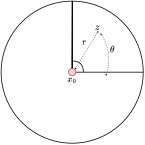
\includegraphics[scale=0.6]{TheorethicalFramework/ND-Laplace/Images/polar-laplace.png}
  \centering
  \caption{Representation of the generated $z = {r \theta}$ and original point $x0$.}
  \label{figure:parea}
\end{figure}

\textbf{Calculating $r$:}
This variable is defined as $dist(x_0, z)$ and can be randomly drawn by inverting the \gls{cdf} for the Laplace distribution:
\begin{equation}
  C{_\epsilon}{^{-1}}(p) = - \frac{1}{\epsilon}(W_-1 (\frac{p - 1}{e}) + 1)
\end{equation}
For this equation, $W_{-1}$ is a Lambert W function with a -1 branch.
\todo[inline]{Explain -1 branch?}
The Lambert w function (also called the product logarithm) is defined as $W(x)e^{W(x)} = x$ \citep{lehtonen_lambert_2016}.
The purpose of the Lambert w function is to invert the \gls{cdf} of the Laplace distribution to generate random noise for one of the coordinates ($r$) using the random value of $p$.

\textbf{Calculating $\theta$:}
The other variable ($\theta$) is defined as a random number $[0, 2\pi]$. \newline
To visualize the data, it is necessary to convert the polar coordinates for $z = (r, \theta)$ back to planar coordinates $z = (x, y)$.
This conversion is described as step 4 of the planar Laplace algorithm \citep{DBLP:journals/corr/abs-1212-1984} and visualized using figure \ref{figure:geo}.
\begin{figure}[h]
  \includesvg[width=0.8\textwidth]{TheorethicalFramework/ND-Laplace/Images/polar-laplace-to-planar.svg}
  \centering
  \caption{Representation of converting the perturbed point $z = (r, \theta)$ to a point ${z_x, z_y}$}
  \label{figure:geo}
\end{figure}

\newpage
\subsection{Truncation} \label{theory:truncation}
After adding the noise to the data, it cannot be ensured the data is within the original domain (figure \ref{figure:truncation-2d}).
If this is not the case, the data is easily distinguished by an unwanted adversary \citep{DBLP:journals/corr/abs-1212-1984,9646489}.
The truncation is an essential part of the mechanism to ensure the data is contained within the domain of the original data $X$.
%We assume a user has a set of data points with a range of [-1, 1].
\begin{figure}[H]
  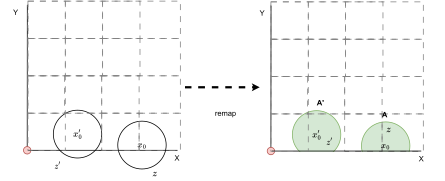
\includegraphics[width=0.7\textwidth]{TheorethicalFramework/ND-Laplace/Images/remapping.png}
  \caption{Representation of truncation of data points for 2-dimensional Laplace mechanism.}
  \label{figure:truncation-2d}
\end{figure}
%A solution was described by Andres et al. in step 5 of the Laplacian mechanism for 2D space \citep{DBLP:journals/corr/abs-1212-1984}.
%A viable solution is to create a grid around the diameter of the set of points $X = R^2$ that belong to the user \citep{DBLP:journals/corr/abs-1212-1984}.
The approach Andres et al. introduces is to remap a perturbed point $z$ to the closest point $x'$ in $G$ \citep{DBLP:journals/corr/abs-1212-1984}.
Here, $G$ is a grid generated using constant cell width.
%Although this approach remaps data within the original domain of $X$, it is not guaranteed it preserves \gls{gi} anymore.
Let the below equation be the collection of probabilities for a point being remapped to a grid cell $x'$ \citep{DBLP:journals/corr/abs-1212-1984}:
\begin{equation}
  R(x) = { y \in R^2 | \forall x' \in G \cdot d(y, x') \leq d(y, x')}
  \label{eq:grid-probability}
\end{equation}
The original \gls{gi} definition contains $K$, which is the probability of $z$ being reported as $x$ (See Equation: \ref{theory:geo-indistinguishability}).
However, this probability is no longer guaranteed because $z$ can also be part of $G$ \citep{DBLP:journals/corr/abs-1212-1984}.
Hence the probability is now $R_X(x) = R(x) \cup X$. \newline
So, the $R_X(x)$ has a different shape depending on the distance $x_0$ and $x'$ (ergo, it depends on the grid cell width). This is due the step units of $G$ stay the same, while the distance $r$ grows \citep{DBLP:journals/corr/abs-1212-1984}.
\newpage
To overcome this issue, Andres et al. propose a way of calculating $\epsilon'$, depending on the step-unit $u$. \citep{DBLP:journals/corr/abs-1212-1984}.
They proved this in theorem 4.1 \citep{DBLP:journals/corr/abs-1212-1984}:
\begin{theorem}[Discretization 2D-Laplace]
  Assume $r_{max} < \frac{u}{\delta_{\theta}}$, and let $q = \frac{u}{r_{max}}\delta_{\theta}$. Let $\epsilon$, $\epsilon' \in R^+$ such that \\
  $\epsilon' + \frac{1}{u}ln \frac{q + 2 e^{\epsilon'u}}{q - 2 e^{\epsilon'u}} \leq \epsilon$ \\
  Then $K_{\epsilon'}$ provides $\epsilon$-geo-indistinguishability within the range of $r_{max}$. Namely, if ${d(x_0, x), d(x'_0, x) \leq r_{max}}$ then: \\
  $K_{\epsilon'}(x_0)(x) \leq e^{\epsilon d(x_0, x'_{0})} K_{\epsilon'}(x'_{0})(x)$.
  \label{theorem:discretization}
\end{theorem}
Here, $\delta_{\theta}$ is the machine's precision, which is the hardware precision of the GPS-location in the context of geographical data. We will omit this in our research, but still provide the full theorem nonetheless. 
The theorem states that $\epsilon'$ is the additional noise needed to satisfy \gls{gi} with the introduction of discretization.
%Then, the final step is truncation based, which is based on the discretization \citep{DBLP:journals/corr/abs-1212-1984}.
It is sufficient to take $r_{max}$ as $diam(X)$, which is the diameter of the set of points $X$ if it satisfies theorem \ref{theorem:discretization} \citep{DBLP:journals/corr/abs-1212-1984}:
So, $r_{max}$ is the maximum distance between points in $X$, which is the area where geo-indistinguishability can be guaranteed \citep{9646489}.

\mycomment{In the context of our research, it is more convenient to find the $u$ based on a given $\epsilon$.
So the challenge is to find the $u$ that satisfies \gls{gi}.
This can be solved by finding the root of the function:
\begin{equation}
  \epsilon' + \frac{1}{u}ln (\frac{\frac{u}{r_{max}} + 2 e^{\epsilon'u}}{\frac{u}{r_{max}} - 2 e^{\epsilon'u}}) - \epsilon = 0
  \label{eq:find-u-with-epsilon}
\end{equation}
The idea of finding the root of a function is to try different values of $u$ until $f(u) = 0$. \todo{Have some proof}
\todo[inline]{Maybe extend this with some more explanation?}}
%This idea was later improved by Chatzikokolakis et al., introducing an optimized way of remapping \citep{chatzikokolakis_efficient_2017}.
%The algorithm uses the Bayesian rule to minimize the loss of utility while remapping the data.
%Instead of remapping to the closest point, it remaps to a location where the loss is minimal.
%To decrease the performance impact of this algorithm, it is possible only to consider a specific region around the perturbed point $z$.
%The disadvantage of this method is the need for a prior set of data points to calculate the optimal remapping.
%It does not work for new users and extends the training period.

\mycomment{\subsection{Optimizing for clustering} \label{2d:optimizing}
The decision of the parameters for the algorithm is straightforward as it depends on the $\epsilon$. \label{paragraph:choosing-r}
This constant is calculated by defining the radius $r$, and the desired level of privacy $l$ and $\epsilon$ is calculated using $l/r$.
The $l$ is a predefined constant $l \in R^+$ but usually will be below 10.
For geographical data, the $r$ can be configured using meters as a unit of measure.
So, for example, $r = 200$ corresponds to a radius of 200m around point $x_0$.
Without a unit, it is a challenge to define a reasonable radius.
%The $\epsilon$ can be considered the inverse unit of $r$ \citep{DBLP:journals/corr/abs-1212-1984}.
In that regard, the radius can also be a flexible value defined based on the crowdedness of a region \citep{chatzikokolakis_constructing_2015}.
Suppose a user's location is within a crowded area.
In that case, the radius can be smaller than if the user is located in a rural area (because the user's location is indistinguishable due to the overlap of other users' locations).
Instead of providing \gls{gi}, the authors introduce a more flexible privacy definition $d_x$-privacy.
The $r$ is calculated based on the mass of other regional locations $r$, which they call \emph{privacy mass}.
So, the total mass of a set A is defined as $M(A) = \sum_{x \in A} m(x) = a + q(x)b$.
Where $m(x)$ is the mass of a location $x$ and $x$ is in value [0, 1].
For this formula, $a$ is the number of points assigned to each location.
The authors define $q(x)$ as the "quality" of a point, which is essentially the number of other users that are also interested in the same point (e.g. a mall).

The $a$ is defined as a Euclidean ball $B_r = {x' | d_{euc}(x, x') \leq r}$, which returns all locations within the radius $r$.
\todo[inline]{Explain this formula better, and create it as a separate equation}
To retrieve a value within [0, 1], the authors use the following formula:
\begin{equation}
  a = \frac{1}{|B_r|}
  \label{equation:privacy-mass-a}
\end{equation}
If the locations are only considered for space and not quality, $q(x)$ is defined as 0 \citep{chatzikokolakis_constructing_2015}.

Although the method is an interesting approach to increasing utility while not reducing privacy, it is hard to adopt for clustering.
For applying it for \gls{ldp}, it is required to supply each user with prior knowledge of the dataset.
This approach would require interaction between data points, hence an interactive setup of the mechanism instead of a non-interactive one. \newline
Nonetheless, the idea of using crowded locations is an exciting approach that is researched further in section \ref{theory:privacy-utility-nd}
}


\newpage
\subsection{Final mechanism}
Finally, we provide as means of a summary the final algorithm for the Laplace mechanism for 2D space
\begin{algorithm}[H]
  \caption{Full mechanism for perturbing training data for planar/2D-Laplace \citep{DBLP:journals/corr/abs-1212-1984}}\label{alg:rq1}
  \begin{algorithmic}
    \Require $X$, $\epsilon$, $u$, $v$ 
    \Ensure $Z$ 
    %\State $r = \frac{\sigma}{2}$ \Comment formula 4.1
    %\State $\epsilon = \frac{l}{r}$ \Comment Calculating privacy budget \citep{DBLP:journals/corr/abs-1212-1984}
    \State Generate $\epsilon'$         \Comment{Theorem: \ref{theorem:discretization}}
    \State $Z \gets \varnothing$
    \State Generate G from given sides $u, v$.
    \State Generate $A$ with acceptable points around $x_0$ 
    \For{$x_i \in X$}
    \State Generate $\theta$       \Comment Equation: \ref{2d:generate-theta}.
    \State Generate the radius $r$ around $x_0$ \Comment Equation: \ref{eq:lambert_w_1}.
    %\State $z_i \gets T(x_{min}, x_{max}, point_i, z_i)$ \Comment algorithm 1.
    \State Convert polar coordinate $(r,\theta)$ to Cartesian coordinates $z = (x, y)$ \Comment Figure: \ref{figure:geo}.
    \If{z $\notin A$}
        \State Remap $z$ to closest point in $A \cap G$. 
    \EndIf
    \State Add $z$ to perturbed set $Z$.
    \EndFor
    \State \Return Z
  \end{algorithmic}
  \label{alg:2d-laplace}
\end{algorithm}
\newpage
\section{3D-Laplace}
The previous sub-section described the use of 2-dimensional noise on geographical data.
This approach has recently been extended to support 3-dimensional data, which benefits indoor navigation \citep{9646489}.
The method is similar to the 2D approach but includes the azimuth angle $\psi$ besides the polar angle $\theta$ and radial distance $r$.

\subsection{Geo-indistinguishability}
To establish the same privacy guarantees for 3-dimensional data as for 2-dimensional data, the original equation \ref{algo:2d-geo-indistinguishability} is extended \citep{9646489}.
\begin{equation}
  K(x_1)(z) \le e^{\epsilon * d_3(x_1, x_2)} K(x_2)(z)
  \label{algo:3d-geo-indistinguishability}
\end{equation}
Where $x_1$ and $x_2$ are two real data points in the same dataset $X$.
%The more $x_1$ and $x_2$ are similar, the more the perturbed location distributions $K(x_1)(z)$ and $K(x_2)(z)$ need to be similar.
\subsection{Spherical Laplace}
The implementation of Min et al. projects the dimensions onto a sphere instead of a circle \citep{9646489}.
This sphere is a unit sphere calculated with a radius of 1.
The polar angle $\theta$ and azimuth angle $\psi$ are randomly calculated based on this sphere. \newline
\textbf{Calculating $\theta$ and $\psi$}: The tuple $U = (\theta, \psi)$ is randomly drawn from the unit sphere using the following equations \citep{9646489}:
\begin{equation}
  \theta = \frac{1}{\pi}
\end{equation}
\begin{equation}
  \psi = \frac{1}{2\pi}
\end{equation}
\textbf{Calculating $r$}: The radial distance $r$ is calculated using the following equation:
\begin{equation}
  r = \frac{1}{2}\epsilon^3 * r^2 * e^{-\epsilon * r}
  \label{eq:3d-laplace-r}
\end{equation}
The gamma scale is the same as for 2D-Laplace but with a shape of 3 instead of 2.
The noise is added to the original location $x$ to obtain the perturbed location $z = x + U*r$.
A clear example of the generated noise by this method is shown in figure \ref{fig:3d-laplace-noise}.
\begin{figure}
  \includegraphics[width=0.6\textwidth]{TheorethicalFramework/ND-Laplace/Images/3d_laplace_noise.png}
  \caption{50 random noise samples generated around point $x_0$ (green dot) using the 3D-Laplace noise method \citep{9646489} plotted on a sphere.}
  \label{fig:3d-laplace-noise}
\end{figure}
Finally, the spherical coordinates are converted to the Cartesian coordinate system to obtain the perturbed location $z$:
\begin{align*}
  z_x = r * \sin(\theta) * \sin(\psi) \\
  z_y = r * \sin(\theta) * \cos(\psi) \\
  z_z = r * \cos(\theta)
\end{align*}
The complete overview is visualized in figure \ref{fig:3d-laplace}.
\begin{figure}
  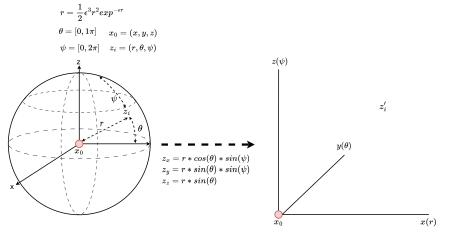
\includegraphics[width=0.8\textwidth]{TheorethicalFramework/ND-Laplace/Images/3d_laplace.png}
  \caption{3D-Laplace noise distribution according to the method proposed by Min et al. \citep{9646489}}
  \label{fig:3d-laplace}
\end{figure}
\newpage
\subsection{Truncation}
As with the 2D-Laplace method, the 3D-Laplace method also needs a truncation method.
This truncation method is also based on the same method as the 2D-Laplace method.
Instead of a plane grid, a cuboid grid is used for 3-dimensional space.
This cuboid remaps the noise to the closest grid cell $g \in G$ or existing point in $X$.
We plotted example data points on a 3-dimensional grid in figure \ref{fig:3d-laplace-example} to demonstrate this:
\begin{figure} [H]
  \includegraphics[width=\textwidth]{TheorethicalFramework/ND-Laplace/Images/example_3d_laplace.png}
  \caption{Applying 3-dimensional noise with $\epsilon = 1$ (red dots) to a dataset $X$ (green dots). Demonstrating remapping to the closest grid point (blue) or $X$.}
  \label{fig:3d-laplace-example}
\end{figure}

\newpage
\subsection{Final mechanism}
Finally, we provide as means of a summary the final algorithm for the Laplace mechanism for 3D space
\todo[inline]{Write down 3D laplace algorithm}
\newpage
\newpage
\section{nD-Laplace}
As mentioned in the previous chapter, the paper that was introduced by Min et al. is be-able to handle 3-dimensional data.
A small recap: a point $(r, \theta, \psi)$ gives us the spherical coordinates of a given 3-dimensional sphere.
An important property for this is the fact that each of these coordinates can be generated separately \citep{DBLP:journals/corr/abs-1212-1984, 9646489}.
The $r$ gives us the radius or distance from $(\theta, \psi)$ to the center of the sphere \footnote{https://mathworld.wolfram.com/SphericalCoordinates.html}.
So, instead of having just these two coordinates, we are be-able to extend this to n-dimensions by considering an n-hypersphere \citep{fernandes_generalised_2019, 9646489}.
To this end, besides points $\theta$ and $\psi$ we also consider $\theta \in S^n$, where S is a unit hypersphere.

The first step to generate the noise is first to select the $r$.
This method is almost identical to the one for 3-dimensional (\ref{eq:3d-laplace-r}).
But, instead of applying a scale of 3, the scale will be $n$ for the number of dimensions in the data \citep{fernandes_generalised_2019}:
\begin{equation}
  \gamma(n, 1/\epsilon)
  \label{eq:nd-laplace-r}
\end{equation}
For the other dimensions, we consider a vector $U = (\theta_1, \theta_2, \theta_n)$ which is uniformly selected based on a unit $n$-hypersphere $S^n$ \citep{fernandes_generalised_2019}.
We consider the work that was proposed by Marsaglia et al. for 4-sphere that can be used for selecting points from an n-hypersphere \citep{marsaglia_choosing_1972}.
This method resolves around selecting points from a hypersphere by using a uniform distribution for the domain [0, 1].
We adopted the approach that uses the Gaussian distribution \footnote{https://mathworld.wolfram.com/SpherePointPicking.html}.

\subsection{Cartesian coordinates}
As with the 2/3D-Laplace, the spherical coordinates need to be converted to Cartesian to be able to cluster.
It is comparable to the way it was done in the previous chapters, however, as there are an $n$-amount of angles the equation is repeated and slightly different:
\begin{align}
  x_1 = r * cos (\theta_1)                                          \\
  x_2 = r * sin (\theta_1) * cos (\theta_2)                         \\
  x_{n} = r * sin(\theta_1) … sin(\theta_{n-2}) *cos (\theta_{n-1}) \\
  x_n = r * sin(\theta_{n-1}) * sin(\theta_{n-2}) * sin(\theta_{n-1})
  \label{eq:nd-laplace-cartesian}
\end{align}
If we combine sections 1 and 2 of this chapter, we are being able to give a good overview of the solution using a similar image as for the 2D and 3D variants (figure \ref{fig:nd-laplace-overview}).
\begin{figure}[H]
  \includesvg[width=0.6\textwidth]{TheorethicalFramework/ND-Laplace/Images/nd_laplace}
  \caption{Overview of the nD-Laplace mechanism}
  \label{fig:nd-laplace-overview}
\end{figure}
\subsection{Privacy versus utility} \label{theory:privacy-utility-nd}
If we continue adding dimensions, we notice the noise is shrinking proportionally.
To understand this behavior, we first have to examine the formula for a hypersphere’s volume.
\begin{equation}
  S_n = \frac{2 \pi^{n/2}}{\gamma(\frac{1}{2}n)}
\end{equation}
Where $\gamma$ is the gamma distribution that is determined based on the number of dimensions $n$ \footnote{https://mathworld.wolfram.com/Hypersphere.html}.
As the amount of dimensions increases, the most volume is located on the hypersphere surface.
When we convert the points to Cartesian coordinates, some will be located at the center (e.g., 0.5), while others will be close to the surface (e.g., 0.0).
However, as the number of dimensions increases, the majority will be close to the surface (e.g., 0.99).
The decreasing amount of volume is illustrated using this figure:
\begin{figure}[H]
  \includegraphics[width=0.8\textwidth]{TheorethicalFramework/ND-Laplace/Images/volume.png}
  \caption{Illustration of the decreasing volume while increasing the number of dimensions}
  \label{fig:curse-of-dimensionality}
\end{figure}

The noise decreases as the dimensions increase, increasing utility.
Hence, it is intriguing to observe the behavior of privacy relative to utility.
This behavior will be further emphasized in a later stage of this research.
\newpage
\subsection{Truncation}
For 2D/3D Laplace, a grid and cuboid were respectively introduced to truncate noise mechanisms \citep{DBLP:journals/corr/abs-1212-1984,9646489}.
This section extends the work done for 2D and 3D Laplace (\ref{theory:truncation}, \ref{2d:optimizing}) \newline
This section introduces an extension for handling any number of dimensions, which can also substitute for 2D/3D.
We want to note that this section focuses on improving utility with remapping.
Any remap function preserves geo-indistinguishability \cite{chatzikokolakis_efficient_2017}, so the required privacy is still preserved.

Recalling both mechanisms, the 2D version operates on a plane and approximates on a grid $G$, while the 3D version works in a 3D space using a cuboid grid.
Given a set of input points $X \subset R^2$, we can truncate points that are outside the domain by remapping them to points within $G$ ($Z = X \cap G$) \citep{DBLP:journals/corr/abs-1212-1984}.
Here, $X$ represents other data points reported locally by the same user.
To extend this approach to n-dimensional data, we need an efficient way to search points in an n-dimensional hypersphere.
To do this, we adopt the idea proposed by Chatzikokolakis et al. of using a kd-tree for efficient searching of the grid \citep{chatzikokolakis_efficient_2017}.
In their research, they describe the utilization of a kd-tree for searching nearby points for a given point.
For this reason, we also use a kd-tree for the following tasks:
\begin{enumerate}
  \item Finding nearby points for $z \in G$ (section: \hyperref[theory:grid-remapping]{Grid with kd-tree remapping}).
  \item Finding nearby points for $x \in X$ and $z \in Z$ (section \hyperref[theory:optimal-remapping]{Optimal remapping}).
\end{enumerate}
For visualization purposes, this section will primarily focus on 2D data.
However, it is important to emphasize that the same algorithm will also be applied to 3D and nD data. The underlying principles and steps of the algorithm remain the same.

We first give an introduction to kd-trees on the next page and then explain how we apply them for the two tasks.

\newpage
\subsubsection*{Kd-trees} \label{theory:kd-trees}
A kd-tree is a algorithm that can be used to search a grid for nearby points \citep{bentley_multidimensional_1975}.
It is capable of doing so, by recursively splitting the grid into a binary tree to search for grid coordinates \citep{washington_k-d_2002}.
In addition to this, it preserves spatial information of the data so it can be utilised to find nearby points using Euclidean distance (nearest neighbor search).
The following example provides an idea on how this works (Figure \ref{fig:kd-tree-theory}):
\begin{figure}[H]
  \includegraphics[width=0.8\textwidth]{TheorethicalFramework/ND-Laplace/Images/kd-tree-part1.png}
  \caption{Representation of constructing a kd-tree with 2 dimensions \citep{washington_k-d_2002}.}
  \label{fig:kd-tree-theory}
\end{figure}
Take, for example, the 2D Laplace algorithm that utilizes a plane (left side).
The data points can be divided based on their x and y coordinates.
Each coordinate becomes a node in the binary tree, and the grid is divided based on these splits.
The binary tree allows us to efficiently search the grid. An expample of this is provided in the following image (Figure \ref{fig:kd-tree-searching-theory}):
\begin{figure}[H]
  \includegraphics[width=0.8\textwidth]{TheorethicalFramework/ND-Laplace/Images/kd-tree-part2.png}
  \caption{Representation of a searching a kd-tree with 2 dimensions \citep{washington_k-d_2002}.}
  \label{fig:kd-tree-searching-theory}
\end{figure}
In the example, we are searching for all points that fall within the radius of a random query point.
Thanks to the grid being divided into a binary tree, a portion of the grid can be efficiently searched, evaluated and referenced.
The biggest advantage is that this greatly reduces the complexity of searching.
Constructing the kd-tree only costs $O(kn)$, where $k$ is the number of dimensions and $n$ is the dataset size.
Searching for a nearest neighbor is a little less efficient, with a time complexity of $O(\log n)$ \citep{washington_k-d_2002}.
A reference to the Big O notation can be found in the attachment \todo{add reference}.
\subsubsection{Grid with kd-tree remapping} \label{theory:grid-remapping}
As explained in the previous paragraph, a kd-tree can be used to perform a nearest neighbor search.
This is highly relevant to our research as it proves to be beneficial for the optimizations we are striving for.
To this end, we adopt this approach for remapping the perturbed datapoints $z \in Z$ to a grid $G$. \newline
We have illustrated the three steps required for this below:
\begin{figure}[H]
  \includegraphics[width=1\textwidth]{TheorethicalFramework/ND-Laplace/Images/KD-tree.png}
  \caption{Representation of a kd-tree with 2 dimensions to remap based on a grid.}
  \label{fig:kd-tree}
\end{figure}
%When using a kd-tree to search for a data point $z_i$, the algorithm begins with an unbalanced binary tree.
%The root is split by the x-axis, and since 4.5 is greater than 3.5, we go to the right.
%This means that we no longer need to consider the left (greyed out) part of the grid.
%We continue traversing the tree until we find the nearest point based on Euclidean distance.
The above illustration presents the grid-remapping algoritm.
Firstly, a grid is generated, where each (blue) point represents the center of a grid cell.
Together, these centroids form the grid dataset, denoted as $G$.
The yellow points and $x_i$ are part of the original collection, denoted as $X$.
Here, $r$ represents the radius used to generate a private version of the data point $x_i$, named $z_i$, based on 2D-Laplace (in this case).
In the illustration, you can observe that $z_i$ falls outside the original domain of $X$, and for this reason, it needs to be remapped.
We accomplish this by utilizing the nearest-neighbor search from the kd-tree algorithm, allowing us to search in $X \cup G$.
Using this algorithm, we can effectively remap point $z \in Z$ to either $X$ or $G$ based on the closest Euclidean distance (Algorithm \ref{alg:grid-remapping-laplace} and Algorithm \ref{alg:find-outside-domain-laplace}).

The utility of this method depends on the number of grid cells in $G$, since a smaller distance will result in more frequent mapping to the surface of the grid.
When $\epsilon$ is very low (and thus farther away), the data points are more likely to map to the grid surface (\ref{fig:3d-laplace-noise}, \ref{fig:3d-laplace-example}).
Increasing the number of grid cells can improve the utility, but this comes at the cost of significantly increased space complexity for $k$ dimensions.
This is because a grid of $n*m$ dimensions has a complexity of $O(n^2)$.
Therefore, we also explore the optimal remapping algorithm proposed by Chatzikokolakis et al \citep{chatzikokolakis_efficient_2017}.
\begin{algorithm}[H]
  \caption{Algorithm for finding points outside the domain of $X$.}
  \begin{algorithmic}
    \Require $x \in X$  \Comment original dataset
    \Require $z \in Z$ \Comment perturbed dataset
    %\State $tree \gets KDTree(X)$ \Comment construct a KDTree from the original data.
    \State $X_{domain} \gets \Call{KDTree::query}{Z}$ \Comment find the closest points.
    \State $X_{features} \gets \Call{List::getfeatures}{X}$ \Comment retrieve dataset dimensions
    \State $X_{outside-domain} \gets []$
    \For{$feature \in X_{features}$} \Comment iterate over all features and check if any points are outside the domain.
    \If{$feature \leq \Call{X::min}{Z} $}
    \State $\Call{row::append}{X_{outside-domain}}$
    \EndIf
    \If{$feature \geq \Call{X::max}{Z} $}
    \State $\Call{row::append}{X_{outside-domain}}$
    \EndIf
    \EndFor
    \State \Return $X_{outside-domain}$ \Comment The index of points outside the domain of $X$.
  \end{algorithmic}
  \label{alg:find-outside-domain-laplace}
\end{algorithm}
\begin{algorithm}[H]
  \caption{Algorithm for generating and remapping to a grid.}
  \begin{algorithmic}
    \Require $x \in X$  \Comment n-dimensional array of original points

  \end{algorithmic}
  \label{alg:grid-remapping-laplace}
\end{algorithm}
\newpage
\subsubsection{Optimal remapping} \label{theory:optimal-remapping}
As we discussed, the remapping will be performance intensive to be-able to provide good utility and that is why we adopt the optimal remapping \citep{chatzikokolakis_efficient_2017}.
Consider the grid that was proposed in \ref{fig:kd-tree}.
After remapping point $z_i$, it is mapped to the center for the grid cell.
Based on the cell width, the distance to the original point $x_i$ and $ z_i$ could be really large.
Our goal is to remap the center of the grid cell (now $z_i$) to a point that is closer to $x_i$ (if applicable). \newline
This is visualized by zooming into the last step of the grid-remapping (Figure \ref{fig:kd-tree}).
\begin{figure}[H]
  %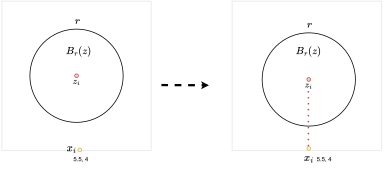
\includegraphics[width=0.7\textwidth]{TheorethicalFramework/ND-Laplace/Images/optimal-remapping.png}
  \includesvg[width=1\textwidth]{TheorethicalFramework/ND-Laplace/Images/optimal-remapping}
  \caption{Representation of optimal remapping \citep{chatzikokolakis_efficient_2017}, where $z_i$ is remapped to $x_i$ using $\sigma(x)$ instead of the center of the grid cell.}
  \label{fig:optimal-remapping}
\end{figure}
In Figure \ref{fig:optimal-remapping} we can observe that $z_i$ is remapped to the center of the grid cell as a consequence of the grid-remapping.
For the reasons mentioned earlier, this is not optimal, and we can further optimize it by utilizing the other data points.
The remapping algorithm works on the idea of crowded places \ref{2d:optimizing}, with the intuition that a crowded place leverages indistinguishability by crowdedness \citep{chatzikokolakis_efficient_2017}.
For the remainder of this thesis, we will use the term "density" instead of "crowdedness" because it better aligns with the clustering of data.

The first step is to calculate $B_r(z)$, which refers to all the data points that fall within the original radius $r$ around the data point $z_i$.
The next step in the algorithm is to collect the data points around $x_i$, in order to calculate how closely it can be remapped to $z_i$ while preserving distinguishability.
This is the collection (convex hull) of all original data points $x \in X$ that are close to $x_i$, determined based on the radius $r$ around $x_i$.
Finally, we combine both sets to obtain $Q_r = B_r \cap X$.
Now that we have the sets of points around $x_i$ and $z_i$, we can calculate the density for each point $q \in Q_r$ \citep{chatzikokolakis_efficient_2017}:
\begin{equation}
  \forall x \in Q_r \quad \sigma(x) = \frac{w(x)e^{-\epsilon d(x, z)}}{\sum{_{q\in Q_r} w(q)e^{-\epsilon d(q, z)}}}
  \label{eq:optimal-remapping-formula-1}
\end{equation}
Where $w(q)$ is the weight of a point $q in Q_r$, and can be seen as points that are visited earlier by the user or other users (e.g. point of interests).
We will revisit this topic in the next paragraph when discussing the practical implementation of the nd-Laplace algorithm.
The same applies to $w(x)$, but for an individual point $q \in Q_r$ instead of the summation.
The outcome of the formula is a collection of values that indicate the degree of density. Which we call $\sigma \in S$.
With this data, we are be-able to calculate a new $z'$ that is closer to $x_i$ to minimize the expected loss of utility \citep{chatzikokolakis_efficient_2017}.

The collection $S$ can be seen as the coefficient for each point $x \in X$, that can be used as a scale to apply for each point $X$ \citep{chatzikokolakis_efficient_2017}:
\begin{equation}
  \bar{\sigma} = \sum_{\sigma \in S} \sigma(x) * x
  \label{eq:optimal-remapping-formula-2}
\end{equation}
Then next, the probabilities are calculated:
\begin{equation}
  W = \forall \sigma \in S = \frac{\sigma(x)}{\bar{\sigma}}
  \label{eq:optimal-remapping-formula-3}
\end{equation}
Finally, the $z'$ is calculated by calculating the average with the probabilities as weight:
\begin{equation}
  z' = \frac{\sum_{weight \in W} x * weight }{\sum_{weight \in W} weight}
  \label{eq:optimal-remapping-formula-4}
\end{equation}
%The first step is to calculate the coefficients for each point $x \in X$ by multiplying the density $\sigma(x)$ with the original point $x$.

%The probability that $z'$ will be closer to $x$ is higher, and this probability is calculated based on the original value $x \in X$ to first determine the coefficient.
%Finally, the new $z'$ is calculated by taking the mean value of $\sigma(x)$ \citep{chatzikokolakis_efficient_2017}.
%As described by chatzikokolakis et al., the 
%Chatzikokolakis et al's work considers a prior set of data point $Q \in R^n$.
%Which are other data points that belong to the user.
%We are interested in the data points that are within the radius $r$ around $z$.
%This is denoted as $B_r(z)$, which is the vector of all points within radius $r$ around $z$.
%In addition to this, there is also a $Q_r$ that is a convex hull of all nearby points.
%Hence, this is described as $Q_r = B_r \cap Q$.
%The final intuition here is that $r$ is automatically generated based on crowdedness (see circle inside figure \ref{fig:optimal-remapping}).
%The last step is to take the mean value of $\sigma(x)$.
%Unfortunately, optimal remapping is not possible for users that do not have sufficient data (e.g. new users).
%The remapping is not applied for these users and is also not applied for $z$ if it is within the domain of $X$.
\subsubsection{Practical implementation}
It is difficult to interpret $w(q) \in Q_r$ beforehand based on other users, as we do not have this information (there is a way, but we explain this at the end of this section).
To this end, we will interpret $w(x)$ as the number of points within the radius $r$ around a point $x \in Q_r$.
Afterwards, it is possible to divide the outcome of this value by the sum of these points (as done in Algorithm \ref{eq:optimal-remapping-formula-1}).
We therefore remain to the same algoritm as proposed by Chatzikokolakis et al. but interpret the weight differently.

It is however still possible to interpret $w(q)$ as the weight based on other user's datapoints.
This requires us to implement the mechanism interactively.
In this approach, all clients perturb their data and sent it to the server.
The server clusters the private data and calculates weight based on cluster information (e.g., crowdedness/density) and shares it with the clients.
The clients then use the optimal remap and share their private information with the server again.
Although this system requires only a single round-trip between server and clients, it reveals cluster information, so we prefer the non-interactive setup.

\begin{algorithm}[H]
  \caption{Algorithm to implement the density remapping of $Z$ to be in the domain of $X$}
  \begin{algorithmic}[1]
    \Require $X, Z, \epsilon$                                \Comment{Requires a truncated nD-Laplace output $Z$}
    \Ensure $Z'$
    \State Filter $Z$ with the data points that were remapped by grid.
    \State Construct a kd-tree from $X$
    \For{$z \in Z$, $x, r \in X$}
    \State Find all points $X_r$ inside radius $r$  around $x$ 
    \State Find all points $B_r$ inside radius $r$ around $z$
    \State $\sigma(x) = []$
    \State $Q_r = X_r \cap B_r$
    \State Count number of points $w_r$ within $Q_r$
    \For{$q \in Q_r$}
    \State Find all points $q$ inside radius $r$ around $q$.
    \State Count number of points $w_q$ within $q$.
    \State Calculate $\sigma(x)$ \Comment Equation \ref{eq:optimal-remapping-formula-1}.
    \State Add $\sigma(x)$ to list
    \EndFor
    \State Calculate $z'$ using $Q_r$ and $\sigma(x)$ \Comment Equation: \ref{eq:optimal-remapping-formula-2}.
    \EndFor
  \end{algorithmic}
  \label{alg:optimal-remapping-laplace}
\end{algorithm}

\begin{itemize}
  \item 1: Receives all the points $z \in Z$ that were originally outside the boundary of $X$ (before remapping).
  \item 2: Constructs a KDTree from the original data $X$, so it can be queried.
  \item 6: Denotes the list of densities for point $x$.
  \item 7: Holds the data-points within the radius $r$ of both $x$ and $z$.
\end{itemize}



\subsection{Putting it together}
\begin{algorithm}[H]
   \caption{Full algorithm for perturbing training data for nD-clustering using nD-Laplace}
   \begin{algorithmic}
      \Require $x \in X$  \Comment n-dimensional array of original points
      \Require $\epsilon$ \Comment privacy budget
      \Ensure $z \in Z$ \Comment n-dimensional array of optimal-remapped perturbed points
      \State $sphere = \Call{GenerateUnitSphere}{x}$ \Comment construct a sphere around $x$.
      \For{$row \in X$}
      \State $d \gets \Call{Length}{row}$ \Comment amount of dimensions
      \State $r \gets \Call{GenerateRadius}{d}$ \Comment Equation \ref{eq:generate_r_for_nd_laplace}.
      \State $sphere \gets \Call{GenerateTheta}{d}$ \Comment Equation \ref{eq:generate_theta_for_nd_laplace}.
      \State $noise \gets \Call{Cartesian}{row, \epsilon}$ \Comment Equation \ref{eq:nd-laplace-cartesian}.
      \State $z = x + noise$
      \State \Call{Append}{$Z, z$}
      \EndFor
      \State \Return Z
   \end{algorithmic}
   \label{alg:nd-laplace}
\end{algorithm}
%\subsection{Extending to $d_x$-privacy}
%\todo[inline]{Find if this is possible}

%Constructing elastic distinguishability metrics for location privacy
\newpage

\subsection{Mechanism overview}
In conclusion, the nD-Laplace mechanism is capable of providing $\epsilon-d_x$-privacy (as well as \gls{gi}) as demonstrated in Formula \ref{theorem:nd-laplace}. The grid-nD-Laplace variant also offers the same privacy guarantee, as proven in Section \ref{section-grid-remapping}. Additionally, the density-nD-Laplace mechanism, being a post-processing step, provides an equivalent level of privacy as nD-Laplace. This equivalence extends to clustering as well \citep{feyisetan_leveraging_2019}.

Furthermore, it is worth noting that the use of kd-trees simplifies the complexity of these variants without compromising their privacy guarantees. Kd-trees serve as a tool to address the search complexity in handling n-dimensional data, rather than directly affecting the privacy assurances.
The following sections will provide a comprehensive framework overview and offer practical insights for its application.

\subsubsection{Flowchart}
All formulas and theories are established for 2D-Laplace, 3D-Laplace, and nD-Laplace, so the mechanism design applies to all three variants:
\begin{figure}[H]
  \includegraphics[width=1.1\textwidth]{TheorethicalFramework//ND-Laplace//Images/overview.png}
  \caption{Non-interactive mechanism design for nD-Laplace.}
  \label{fig:final-mechanism-design}
\end{figure}
%\todo[inline]{Modify to density-nD-Laplace \& nD-Laplace for image reporting}
For easy navigation, we provide a list of all algorithms:
\begin{enumerate}
  \item Based on the number of dimensions, the algorithm decides the correct Laplace mechanism to use:
        \begin{itemize}
          \item 2D-Laplace:  Algorithm: \ref{alg:2d-laplace}
          \item 3D-Laplace:  Algorithm:\ref{alg:3d-laplace}
          \item nD-Laplace: Algorithm: \ref{alg:nd-laplace}
        \end{itemize}
  \item Grid remapping: Section:\ref{section-grid-remapping}
  \item Density remapping: Algorithm: \ref{alg:optimal-remapping-laplace}
\end{enumerate}
In addition, relevant research questions are incorporated into the architecture overview.
These questions are covered in chapter \ref{chapter:methodology}.
\subsubsection{Practical example}
The shape of the dataset is necessary for the usefulness of clustering.
With our algorithm, there are four different shapes/variants of the dataset.
For example, this has been visualized using a 2D dataset based on the Circle dataset (\ref{datasets-section}).
Our mechanism aims to provide privacy and preserve the dataset its shape to benefit the utility of clustering.
Grid remapping and density remapping are used to achieve this goal.

\begin{figure}[H]
  \includegraphics[width=1.1\textwidth]{TheorethicalFramework//ND-Laplace//Images/output.png}
  \caption{Example of optimal remapping for the 2-dimensional Circle dataset. The example shows the different steps of the mechanism in sequence for a dataset perturbed with a privacy budget of 0.5.}
\end{figure}
\begin{enumerate}
  \item Dataset: the blue dots represent the original dataset without any modifications.
  \item Adding noise: the green crosses represent the dataset after adding noise; for this particular example, this is 3D-Laplace (Algorithm \ref{alg:3d-laplace}):
        As can be observed, the data is generated from the center, causing many data points to fall outside the original domain of the dataset.
  \item Grid-remapping: the red dots represent the dataset after grid-remapping (Section \ref{section-grid-remapping}).
        After performing the grid remapping algorithm, all points outside the data domain are remapped to be within the domain. The data-shape is also partly restored. 
  \item Optimal-remapping: the green dots represent the dataset after optimal-remapping (Algorithm \ref{alg:optimal-remapping-laplace}). As can be observed, this process is primarily focused on achieving a better utility by reproducing the original shape.
\end{enumerate}


\chapter{Methodology}

To gain insights into the proposed methods for researching the appliance of (ND)-Laplace for cluster algorithms we conducted experiments.
The experiment results are used to evaluate our method against other literature.
In this chapter we explain:
\begin{enumerate}

  \item Datasets
  \item Environmental setup.
  \item For each research question: Description of the different experiments.
  \item For each research question: Results.
\end{enumerate}

\section{Datasets}
For this research, we will use a synthetic dataset for all three research questions.
%In addition to this, we used the LSun dataset as a lot of comparable literature uses this as well for evaluation.
%\todo[inline]{Describe LSun dataset}
% Please add the following required packages to your document preamble:
% \usepackage{booktabs}
\begin{table}[h]
  \begin{tabular}{@{}llllll@{}}
    \toprule
    Dataset & Records & Centers & Dimensions & Standard deviation & Research \\ \midrule
    1       & 50      & 4       & 2          & 0.60               & RQ 1     \\ \bottomrule
    2       & 50      & 4       & 3          & 0.60               & RQ 2     \\ \bottomrule
    3       & 50      & 4       & 5          & 0.60               & RQ 2     \\ \bottomrule
  \end{tabular}
\end{table}
Research question 3 uses a "real-world" dataset to properly assess the different dataset properties that are the subject of this research question.

\section{Environmental setup}
For running the experiments we make use of 16GB ram memory and i7-10750H 2.6Ghz processor.
The experiments are run using a Docker container which runs a pre-configured distribution of Linux Alpine.
It includes a pre-installed Anaconda environment for python \footnote{https://github.com/devcontainers/images/tree/main/src/anaconda}\footnote{tag: mcr.microsoft.com/devcontainers/anaconda:0-3}.
We run the container using the dev-container feature for visual-studio code \footnote{https://code.visualstudio.com/docs/devcontainers/containers}.
This allows us to create a reproducible experiment environment.
\newpage
\subsection{Libraries \& code versions}
We use python version 3.9.13 with Jupyter notebook for creating a reproducible experimental environment.
The packages for python are:
\begin{enumerate}
  \item Scikit-learn: 1.0.*
  \item Yellow-brick: 1.5
  \item Numpy: 1.24.*
  \item Pandas: 1.4.*
  \item Seaborn: 0.11.*
  \item Mathplotlib: 3.5.*
\end{enumerate}

\section{Methods}
This section explains what methods/ algorithms we used and how we evaluate them.
\subsection{Clustering methods}
For the three different algorithms: K-Means, \gls{ap} and \gls{dbscan} we analyzed the most important decisions regarding parameter selection.
In this section, we give a short list and explanation of the different parameters we used throughout the experiments.
For all three Sklearn was used, and for each of them we also provide the underlying formula.
\subsubsection{K-Means}
\todo[inline]{Work in progress}
\begin{equation}
  \sum_{i=0}^{n}\min_{\mu_j \in C}(||x_i - \mu_j||^2)
\end{equation}
\begin{table}[h]
  \begin{tabular}{|l|p{6cm}|l|l|}
    \hline
    Parameter & Description                          & Value & Dataset   \\ \hline
    K-value   & Calculated based on an "elbow" plot. & 4     & Dataset 1 \\ \hline
    K-value   & TODO                                 & ??    & Dataset 2 \\ \hline
    K-value   & TODO                                 & ??    & Dataset 3 \\


    \hline
  \end{tabular}
  \caption{K-Means hyperparameters for dataset 1 - 3}
  \label{tab:kmeans-formula-dataset-2}
\end{table}

\subsubsection{Affinity Propagation}
\todo[inline]{Work in progress}
\begin{table}[h]
  \begin{tabular}{|l|p{6cm}|l|l|}
    \hline
    Parameter      & Description                                                                                & Value & Dataset   \\
    \hline
    Preference     & We decided to use the median similarity as described in section \ref{theory:clustering-ap} & TODO  & dataset 1 \\
    \hline
    Preference     & ""                                                                                         & TODO  & dataset 2 \\
    \hline
    Preference     & ""                                                                                         & TODO  & dataset 3 \\
    \hline
    Damping factor & For now it is kept at the default value (\ref{theory:clustering-ap})                       & 0.5   & dataset 1 \\
    \hline
    Damping factor & ""                                                                                         & 0.5   & dataset 2 \\
    \hline
    Damping factor & ""                                                                                         & 0.5   & dataset 3 \\
    \hline
  \end{tabular}
  \caption{Affinity Propagation hyperparameters for datasets 1 - 3}
  \label{tab:ap-formula-sklearn}
\end{table}
\newpage
\subsubsection{DBSCAN}
\begin{table}[h]
  \begin{tabular}{|l|p{6cm}|l|l|}
    \hline
    Parameter      & Description                                                                                                    & Value & Dataset   \\
    \hline
    Epsilon        & Decided using the k-distance plot                                                                              & TODO  & Dataset 1 \\
    \hline
    Epsilon        & ""                                                                                                             & TODO  & Dataset 2 \\
    \hline
    Epsilon        & ""                                                                                                             & TODO  & Dataset 3 \\
    \hline
    Minimum points & Decided using the formula $minPts = n * 2$, where n is the number of features (\ref{theory:clustering-dbscan}) & 4     & Dataset 1 \\
    \hline
    Minimum points & ""                                                                                                             & 6     & Dataset 2 \\
    \hline
    Minimum points & ""                                                                                                             & 10    & Dataset 3 \\
    \hline
  \end{tabular}
  \caption{DBSCAN  hyperparameters for datasets 1 - 3}
  \label{tab:dbscan-formula-sklearn}
\end{table}

\subsection{Evaluation}
With differential privacy, it is a trade-off of utility versus privacy.
Therefore, for the evaluation of the 2D/3D-Laplace algorithms, we compare both criteria to achieve a consensus between utility and privacy.
\subsubsection{Utility}
Based on chapter \ref{theory:evaluate}, we can conclude that the corresponding literature mainly evaluates one clustering algorithm and not multiple ones.
Because of this, we do not use any internal validation; because the different types of metrics are too easily influenced by the choice of clustering algorithm.
Instead, we decided to pick up external validation methods similar to other studies as well.
They did use either Rand Index or Mutual Information, but because both have different strengths we evaluate both.

It is not likely that we will use many data points for research questions 1 and 2.
To compensate for this, the adjusted version is used for both Rand Index and Mutual Information.
Since both Mutual Information and Rand Index have different characteristics in the type of clustering algorithm, we use both.
%The clustering algorithm is trained using the plain data and functions as the ground truth \citep{9646464,sun_distributed_2019}.
%Because of this, we are being able to calculate the \gls{ami} and compare the centroids between the non-private and privately trained clusters.
To reduce the possible bias of results we executed them 10 times for multiple privacy budgets and report the average for each \citep{9679364}.

Finally, the implementation for these metrics is provided by the Scikit-learn package.
With the underlying formulas:
\begin{equation}
  AMI(U, V) = \frac{MI(U, V) - E(MI(U, V))}{avg(H(U), H(V)) - E(MI(U, V))}
\end{equation}
\capequation{Adjusted Mutual Information formula \citep{vinh_information_nodate-2,hubert_comparing_1985-1}}
\begin{gather}
  RI = \frac{a + b}{C^{n}_{2}} \\
  ARI = \frac{RI - E(RI)}{max(RI) - E(RI)}
\end{gather}
\capequation{(Adjusted) Rand Index formula \citep{rand_objective_1971, hubert_comparing_1985-1}}

%%The second way to measure utility is to calculate the error between the non-private and perturbed data \citep{9679364,sun_distributed_2019,xia_distributed_2020-1}.
%There are several methods to do this (See \ref{theory:evaluate}), but we use the \gls{aee}.
%As with \gls{ami} we run the calculations for multiple privacy budgets 10 times and report the average for each budget.
%\todo[inline]{Explain why AEE and not RE}

\subsubsection{Privacy}
The most important one here is the preserving of \gls{gi} according to the formula \ref{algo:2d-geo-indistinguishability}.
This validates that we applied the algorithms in the right way and automatically inherit the strong privacy guarantees provided by \gls{gi}.
A disadvantage of this method is that it cannot be used to achieve a clear representation of privacy (it is either "yes" or "no").
Therefore, we also will analyze the average Euclidean distance the differential privacy provides for each epsilon.

%Therefore, we analyze our method according to a popular attack: Membership inference attack.

%For this purpose, we make use of a black-box Member inference attack, called "HopSkipJump" \citep{chen_hopskipjumpattack_2020,li_membership_2021}.
%This attack is evaluated using a semi-supervised setup, as proposed in this figure: \ref{fig:unsupervised-mia-attack}.
%We will make use of a decision tree model for classification but can be replaced by any other classification model.
%Both the private and non-private trained models are evaluated based on the true positive rate (TPR) and false positive rate (FPR).
%Respectively meaning, the TPR is higher if the MIA is successful and likewise the FPR if the MIA is unsuccessful.
%We hypothesize that the private model leverages a higher FPR in comparison to the non-private variant.

%Therefore, it is more convenient to apply the geo-indistinguishability as an error metric provided in \ref{eq:geo-as-an-error}.

\subsection{Scaling}
Because we use a distance metric, we need to apply some data standardization.
For this purpose, we use standard scaling provided by the Scikit-learn package \footnote{https://scikit-learn.org/stable/modules/preprocessing.html}.
This is only for clustering, so it is applied after all the perturbation algorithms.
\subsection{Research question 1}

\mycomment{
  We propose several solutions for open issues based on the theoretical framework. \newline
  \subsubsection{Choosing r: } Based, on the idea of chatzikokolakis et al. to lower the size of the radius if the place is crowded, we can do the same with clustering.
  For this, we could use a metric like the standard division.
  This metric does exactly this, by providing the deviation from the mean:

  This metric increases based on clutteredness of the data, which allows us to generate a radius $r$ automatically regardless of domain.
  Therefore, we depend on the configurability of epsilon entirely on privacy level $l$.
  The generic standard deviation can be defined as:
  \begin{equation}
    \sigma = \sqrt{\frac{\sum{(x_i - \mu)^2}}{n}}
  \end{equation}
  The $\sigma$ being our diameter $d$, the radius $r$ is then calculated as $\frac{d}{2}$. \newline
}
\subsubsection{Truncation: }
We explained the theory for truncation earlier in paragraph \ref{theory:truncation}.
The methods proposed work correctly for a geographic map where other (historic) locations for remapping are available.

However, it is difficult to apply this to data clustering.
The number of data points is not known beforehand, so we may remap to a location that is too far away.
This way we lose important distance information, which hurts the clustering.
Also, the truncation threshold is so clear (the points are outside the known 2D domain), that we do not have to rely on historical data for remapping.
Our algorithm can be much simpler by re-calculating the noise until it will be within the domain:
\mycomment{
  \begin{equation}
    T(x_{max}, x_{min}, z, x_0) \begin{cases} z &\text{if } 0 < 1 \\ T(x_{max}, x_{min}, planarLaplace(epsilon, x_0), x_0)  &\text{else} \end{cases}
  \end{equation}
}
\begin{algorithm}[H]
  \caption{Truncation algorithm ($T(\min, \max, x_0, z)$) for clustering with planar Laplace}\label{alg:truncaction-rq1}
  \begin{algorithmic}
    \Ensure $z$
    \State $x_1, y_1 \gets x_{min}$
    \State $x_2, y_2 \gets x_{max}$
    \State $z_x, z_y \gets z$
    \If{$x_1 < z_x < x_2$ and $y_1 < z_y < y_2$}
    \State \Return $z$
    \Else
    \State $x, y \gets x_0$
    \State $z_2 \gets LP(\epsilon, x, y)$ \Comment See formula 3.3.
    \State \Return $T(x_{min}, x_{max}, x_0, z_2)$ \Comment Rerun recursively
    \EndIf
  \end{algorithmic}
\end{algorithm}
This algorithm uses $x_{min}$ and $x_{max}$ to re-calculate the points within the domain using respectively the minimum X/Y and maximum X/Y.
An example of this is visualized:
\begin{figure}[h]
  \includegraphics[width=0.8\textwidth]{Method/images/truncation-rq1.png}
  \label{fig:truncation}
  \centering
  \caption{Representation of the remapping algorithm for clustering for points $z_3$ and $z_4$ }
\end{figure}

%\subsubsection{Probability metric $K(x)(Z)$}
%\todo[inline]{Explain the probability metric $K$ we used}

%\newpage
\subsubsection{Algorithm}
The full algorithm for the perturbation:
\input{Method/algorithms/rq1.tex}
%% We apply the theory for planar laplace proposed by \citep{DBLP:journals/corr/abs-1212-1984}

\subsection{Research question 2}
\todo[inline]{Starts after RQ1}
\subsection{Research question 3}
\todo[inline]{Starts after RQ2}

%\input{Chapter2/chapter-2}

%\input{Chapter3/chapter-3}

%\input{Chapter4/chapter-4}

%\input{Chapter5/chapter-5}

%\input{Chapter6/chapter-6}



\backmatter
\pagenumbering{roman}

\bibliographystyle{plainnat}
\bibliography{report}

%% Use letters for the chapter numbers of the appendices.
%\appendix
\appendix
%  \chapter{Hyperparameters}
\section{K-Means}
For selecting the appropriate amount of clusters, we used an "elbow" plot in combination with the silhouette score.
\begin{enumerate}
  \item Dataset 1: 4 clusters (see figure: \ref{hyperparameters:k-means-dataset1})
  \item Dataset 2: TODO
  \item Dataset 3: TODO
\end{enumerate}
\begin{figure}
  \includegraphics{Appendix/parameter-selection/selecting-k.png}
  \caption{Selecting the $k$ for K-Means for dataset 1 using the "elbow plot" using section \ref{theory:kmeans}}
  \label{hyperparameters:k-means-dataset1}
\end{figure}
\section{DBSCAN}
For the selection of the appropriate epsilon, we used the k-distance plot.
\begin{enumerate}
  \item Dataset 1: 0.9 epsilon (see figure: \ref{hyperparameters:DBSCAN-dataset1})
  \item Dataset 2: TODO
  \item Dataset 3: TODO
\end{enumerate}

\begin{figure}
  \includegraphics{Appendix/parameter-selection/selecting-eps.png}
  \caption{Selecting the $\epsilon$ for DBSCAN for dataset 1 using the "k-distance plot" using section \ref{theory:clustering-dbscan}}
  \label{hyperparameters:DBSCAN-dataset1}
\end{figure}
%  \input{Appendices/appendix-b}
%  \input{Appendices/appendix-c}

\printglossaries
\end{document}
